\documentclass[a4paper,11pt]{article}
\usepackage{graphicx}
\usepackage{onecolpceurws}
\usepackage{url}
\usepackage{hyperref}

\title{The TTC 2014 Movie Database Case}

\author{
Tassilo Horn\\ University of Koblenz-Landau\\ Germany\\ horn@uni-koblenz.de
\and
Christian Krause\\ SAP Innovation Center\\ Germany\\ christian.krause01@sap.com
\and
Matthias Tichy\\ Chalmers $|$ University of Gothenburg, Sweden \\matthias.tichy@cse.gu.se
}
\newcommand{\p}[1]{\textsf{\small #1}}

\institution{}

\begin{document}
\maketitle

\begin{abstract}
  Social networks and other web 2.0 platforms use huge amounts of data to offer
  new services to customers. Often this data can be expressed as huge graphs
  and thus could be seen as a potential new application field for model
  transformations. However, this application area requires that model
  transformation tools scale to models with millions of objects. This
  transformation case targets this application area by using the IMDb movie
  database as a model. The transformation deals with identifying all actor
  couples which perform together in a set of at least three movies.
  \end{abstract}
\vskip 32pt


\section{Introduction (MTT)}

The driving force behind social networks and other new web 2.0
offerings is often huge amount of data. Consequently, concepts like
MapReduce \cite{Dean08} and libraries like Hadoop \cite{Hadoop} and
Giraph \cite{Giraph} have been developed to efficiently process these
huge amount of data. However, model transformation approaches have so
far not adressed this field.

Automotive software is an already well-established application field
for model-driven software engineering and its models also approach
huge sizes. As a consequence from these two examples, model
transformation approaches must be scalable to models with million
objects to be applicable for these application areas.

We present in the following a case which uses the IMDb movie database
\cite{IMDBDATA} as a data source. The IMDb movie database contains information
about movies, actors performing in the movies, movie ratings, etc. The main
task is to develop a model transformation which identifies \emph{all} couples
of two actors who perform in at least three common movies and calculate the
average rating of those movies.  This core task is then generalized to cliques
of \(n\) actors.  Furthermore, some queries calculating top-ten lists of
couples and cliques are to be written.  Evaluation criteria are correctness and
performance.

In the following section, we describe the case in more detail
including the meta model as well as the different basic and extension
tasks. After that, Section \ref{sec-eval} presents the evaluation
criteria for submitted solutions to this case.


\section{Detailed Case Description (MTT)}\label{sec-case}

We use the IMDb data about movies, actors, actresses and movie ratings for this
transformation case. The resulting metamodel is shown in
Figure~\ref{fig:metamodel}. In addition to the obvious classes, the metamodel
contains a common superclass for actors and actresses as well as classes for
groups of actors which play in common movies. The class \p{Group} contains the
attribute \p{avgRating} which stores the average rating of the common movies of
the group of actors. The metamodel distinguishes between groups of two persons
(a \p{Couple}) or a \p{Clique} of $n$ persons to support the different
tasks in this transformation case.  

\begin{figure}[ht]
\centering
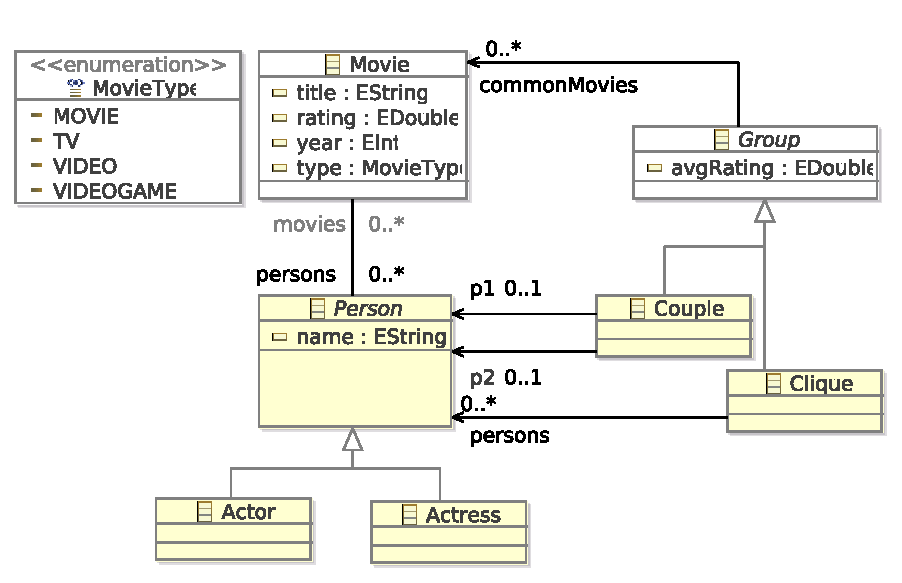
\includegraphics[width=0.6\textwidth]{movies}
\caption{A metamodel for the relevant aspects of the movie database}
\label{fig:metamodel}
\end{figure}

The EMF model as well as a parser for the
IMDb database files is available at \cite{IMDB2EMF}. The pre-parsed
IMDb models are available on request. The transformation case will use
synthetic data (as generated in Task 1) for the evaluation of
the correctness of the submitted transformations as well as real data
from IMDb for the performance evaluation.


\subsection{Task 1: Generating Test Data (CK)}
\label{sec:gen-test-data}

%% Notes from Tassilo:
%%
%% - The test data generation currently creates models contains only couples.
%% For the extension tasks it would be good if the rules also created cliques
%% of size 3, 4, and 5.  The real data does contain such cliques, but finding
%% those is extremely costly.  Therefore, we should be able to validate
%% solutions for the extension tasks also with just the simpler, smaller
%% generated models.
%%
%% - The test data generation should also assign unique names to the Actors and
%% Actresses, and ratings to the Movies.  Else, the computation of the average
%% rating and the top-ten queries cannot be evaluated with the test models.
%% (Again, the real IMDb models are probably to complex/large for most
%% participants.)

The goal of this task is to generate (synthetic) test data which will be used
later to evaluate the correctness and the performance of the solution of the 
main task. The transformation to be implemented takes an empty model and 
generates a number of movies, actresses, actors and references between them.
The number of objects to be generated is determined by an integer-valued 
runtime parameter $n\geq0$. Specifically, the transformation is supposed
to generate $5n$ actors, $5n$ actresses and $10n$ movies, totalling in 
$20n$ nodes. For every generated actor and actress a unique name, and for 
every movie a rating is derived from $n$. Additionally, the references between
persons and movies are generated in a specified way.

The specific patterns to be generated are shown in the Henshin~\cite{ABJ+10} rules in
Figure~\ref{fig:gen-test-data}. Each of the two used rules generates five
persons and five movies. The movie ratings and the name of the persons are
derived from $n$. The five persons in the rule \textsf{createPositive} play
together in three movies. In contrast,
every possible pair of persons generated by the rule \textsf{createNegative}
plays together in at most two movies.

For the following tasks, test data should be generated for different values 
of $n$ which can be found in Table~\ref{tab:synthetic-numbers}.


\begin{figure}[p]
\centering
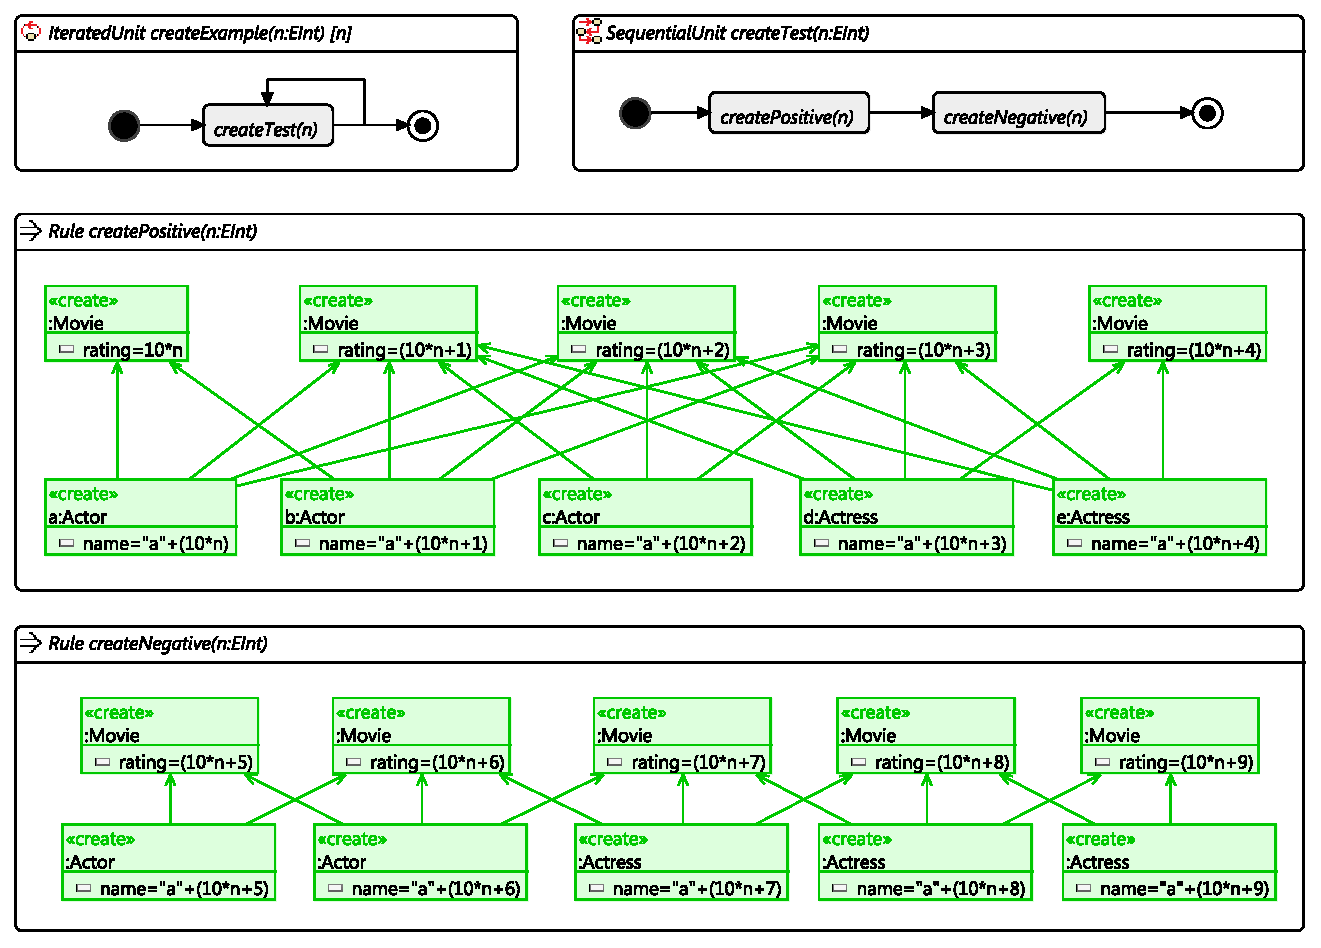
\includegraphics[scale=1.0,angle=90]{gen-test-data3}
\caption{Henshin specification for generating synthetic movie test data.}
\label{fig:gen-test-data}
\end{figure}

\subsection{Task 2: Finding Couples (CK)}

In this task, a transformation shall be implemented that takes a graph
consisting of inter-connected movies, actors and actresses as input, and
creates additional nodes and links in this graph.\footnote{Both in-place and
  out-place transformation approaches are possible.} Specifically, the task is
to find all pairs of persons (actors or actresses) which played together in at
least three movies.  For every such pair, the transformation is supposed to
create an object of type \textsf{Couple} referencing both persons using the
\verb|p1| and \verb|p2| references, and referencing all movies in which
\emph{both} persons played in using the \verb|commonMovies| reference.


\subsection{Task 3: Computing Average Rankings (CK)}

The input model of this task is the one generated in Task 2,
i.e., a graph consisting of movie, actor, actress and couple
nodes. The goal of this task is to set the \verb|avgRating|-attribute
of all couple nodes to the average (i.e. the
arithmetic mean) of the ratings of all movies that
\emph{both} persons played in.

\subsection{Extension Task 1: Compute Top-Ten Couples (TH)}

The goal of this task is to produce top-ten lists of the couples created by
Task~2.  For this purpose, two model queries should be given.

\begin{enumerate}
\item[(a)] Compute the top-ten couples according to the average rating of their
  common movies (requires Task~3 to be solved).
\item[(b)] Compute the top-ten couples according to the number of common
  movies.
\end{enumerate}

Each of the couples in the top-ten lists should be printed with the names of
the two persons, the average rating (only if Task~3 has been solved), and the
number of the couple's common movies.  We don't require printing the common
movies' titles because the couple with the most common movies in the complete
IMDb model has more than 400 of them.

If two couples have the same value for the average rating/number of common
movies, their order in the top-ten list is arbitrary.  However, an extra bonus
point can be earned by cutting those ties in a stable manner, for example by
applying the respective other metric in that case.  E.g., when computing metric
(a) and two couples have the same average rating, then the one with more common
movies could be listed first.  If both values are equal, one could fall back to
comparing hash-codes or the names of the members of the couples.

\subsection{Extension Task 2: Finding Cliques (TH)}

This extension task is a generalization of Task~2.  A clique is a group of at
least \(n\) persons (with \(n \geq 3\)) acting together in at least 3 movies.
So a couple is essentially a clique of size \(n = 2\).

The extension task is to find cliques of a given size \(n\), and to create a
\verb|Clique| element for each of them referencing the clique's members, and
its common movies like the couples in Task~2.

The task will be evaluated for \(n \in \{3, 4, 5\}\), so it can be solved by
writing three similar rules manually.  However, to achieve a full completeness
score for this task, a solution should work for any \(n \geq 3\).  Therefore, a
transformation could have \(n\) as a parameter, or there could be a
higher-order transformation that receives \(n\) and generates a rule creating
cliques of exactly that size.

It would be interesting to be able to specify the required number of common
movies \(c\) freely.  By default and according to Task~2, \(c\) is fixed to 3.
You can earn an extra bonus point if \(c\) may be customized.


\subsection{Extension Task 3: Compute Average Rankings for Cliques (TH)}

Like it was done for couples in Task~3, the \verb|avgRating| attribute of
cliques should be set to the average rating of all its common movies.

\subsection{Extension Task 4: Compute Top-Ten Cliques (TH)}

This is a variant of Extension Task~1 for cliques instead of couples.  Again,
two queries should be given.

\begin{enumerate}
\item[(a)] Compute the top-ten cliques of a given size \(n\) according to the
  average rating of their common movies (requires Extension Task~3 to be
  solved).
\item[(b)] Compute the top-ten cliques of a given size \(n\) according to the
  number of common movies.
\end{enumerate}

Again, every clique should be printed with the names of its members, the
average rating, and the number of common movies.  Like in Extension Task~1, an
extra bonus point can be earned by cutting ties in a stable manner.


\section{Evaluation Criteria (MTT)}\label{sec-eval}

The evaluation of the submitted transformation will be done on
synthetic data as well as real data from the IMDb database. The IMDb
database is regularly updated. In order to provide a common set of
data, we provide the IMDb database in a version from December 2013 to
participants by request. 

\subsection{Correctness Tests (TH)}

Correctness is checked using the synthetic data.

We provide: number of couples and top ten lists.

\subsection{Benchmarks (CK)}

The goal of this task is to generate a performance benchmark
of your solutions to Task 2 and 3. These benchmarks should be
executed using two different sets of input data:
\begin{enumerate}
\item[(a)] synthetic test data generated using the transformation for Task 1, 
\item[(b)] provided data from the IMDb movie database (available at \cite{IMDBDATA}; parsable, e.g., using \cite{IMDB2EMF}).
\end{enumerate}
For both cases, you should run the transformations for Task 2 and 3
separately and measure the time needed to complete the transformation 
(without loading and saving the model).
If you solved also the extension tasks, please also generate benchmarks
for these cases.

%% Tassilo: Why not measuring Task 2 on its own?

In order to evaluate the scalability of the solution, you should
increase the input model size in equal step sizes, e.g. by 
100000 nodes. For the synthetic test data, the parameter can be
set to $n=5000, 10000, 15000\ldots$ to achieve this. For the
real data from the IMDb database, we compiled about 30 input 
models of different sizes that you should use.
We recommend plotting the run-times using charts where
the x-axis refers to the size of the input model in number of nodes,
and the y-axis shows the execution times (e.g. in seconds).


\bibliographystyle{plain}
\bibliography{biblio}

\appendix



\section{Expected Number of Couples and Cliques}
\label{sec:expected-numbers}

\begin{table}[h!]
  \centering
  \begin{tabular}{| l | r | r | r | r |}
    \hline
    \textbf{Model (\(n\))} & \textbf{\#Couples} & \textbf{\#Triples} & \textbf{\#Quadruples} & \textbf{\#Quintuples}\\
    \hline
    1000   & 10000   & 10000   & 5000    & 1000\\
    2000   & 20000   & 20000   & 10000   & 2000\\
    3000   & 30000   & 30000   & 15000   & 3000\\
    4000   & 40000   & 40000   & 20000   & 4000\\
    5000   & 50000   & 50000   & 25000   & 5000\\
    10000  & 100000  & 100000  & 50000   & 10000\\
    50000  & 500000  & 500000  & 250000  & 50000\\
    100000 & 1000000 & 1000000 & 500000  & 100000\\
    200000 & 2000000 & 2000000 & 1000000 & 200000\\
    \hline
\end{tabular}
\caption{The synthetic models with the expected numbers of Couples and Cliques of various sizes}
\label{tab:synthetic-numbers}
\end{table}


\begin{table}[h!]
  \centering
  \begin{tabular}{| l | r | r |}
    \hline
    \textbf{Model}              & \textbf{\#Couples} & \textbf{\#Triples}\\
    \hline
    imdb-0005000-49930.movies   & 17352              & 127825\\
    imdb-0010000-98168.movies   & 28211              & 188712\\
    imdb-0030000-207420.movies  & 35198              & 200532\\
    imdb-0045000-299504.movies  & 43294              & 210985\\
    imdb-0065000-404920.movies  & 57889              & 220891\\
    imdb-0085000-499995.movies  & 79470              & 243314\\
    imdb-0105000-591042.movies  & 104479             & 276499\\
    imdb-0130000-709551.movies  & 136956             & 307405\\
    imdb-0150000-796950.movies  & 164463             & 340755\\
    imdb-0175000-901769.movies  & 208155             & 427824\\
    imdb-0200000-1004463.movies & 244627             & 457833\\
    imdb-0225000-1096479.movies & 298390             & 594032\\
    imdb-0255000-1204331.movies & 361858             & 721604\\
    imdb-0280000-1296503.movies & 408151             & 781216\\
    imdb-0310000-1402659.movies & 508839             & 1346807\\
    imdb-0340000-1505143.movies & 585689             & 1469156\\
    imdb-0370000-1603848.movies & 653715             & 1544170\\
    imdb-0400000-1702751.movies & 740961             & 1660769\\
    imdb-0430000-1793844.movies & 829136             & 1892483\\
    imdb-0465000-1904728.movies & 930509             & 2043816\\
    imdb-0495000-2000900.movies & 1017752            & 2173809\\
    imdb-0525000-2098976.movies & 1113226            & 2332100\\
    imdb-0560000-2205192.movies & 1222959            & 2525431\\
    imdb-0590000-2293503.movies & 1309101            & 2684821\\
    imdb-0625000-2397550.movies & 1441850            & 3656513\\
    imdb-0660000-2501893.movies & 1562317            & 3953798\\
    imdb-0695000-2605751.movies & 1687269            & 4253567\\
    imdb-0725000-2696312.movies & 1805982            & 4677444\\
    imdb-0760000-2800659.movies & 2034680            & 5403338\\
    imdb-0795000-2904388.movies & 2166743            & 5724736\\
    imdb-0830000-3003237.movies & 2308300            & 6148282\\
    imdb-0865000-3097577.movies & 2434934            & 6453770\\
    imdb-0900000-3193920.movies & 2558365            & 6773334\\
    imdb-all-3257145.movies     & 2709371            & 8227081\\
    \hline
  \end{tabular}
  \caption{The IMDb Models with the expected numbers of Couples and Triples (Cliques of size 3)}
  \label{tab:imdb-numbers}
\end{table}

\section{Expected Top-Ten Lists}
\label{sec:expected-top-ten}



\end{document}


